\documentclass[a4paper,12pt]{article}
%%%%%%%%%%%%%%%%%%%%%%%%%%%%%%%%%%%%%%%%%%%%%%%%%%%%%%%%%%%%%%%%%%%%%%%%%%%%%%%%%%%%%%%%%%%%%%%%%%%%%%%%%%%%%%%%%%%%%%%%%%%%%%%%%%%%%%%%%%%%%%%%%%%%%%%%%%%%%%%%%%%%%%%%%%%%%%%%%%%%%%%%%%%%%%%%%%%%%%%%%%%%%%%%%%%%%%%%%%%%%%%%%%%%%%%%%%%%%%%%%%%%%%%%%%%%
\usepackage{eurosym}
\usepackage{vmargin}
\usepackage{amsmath}
\usepackage{graphics}
\usepackage{epsfig}
\usepackage{subfigure}
\usepackage{enumerate}
\usepackage{fancyhdr}
\usepackage{framed}

\setcounter{MaxMatrixCols}{10}
%TCIDATA{OutputFilter=LATEX.DLL}
%TCIDATA{Version=5.00.0.2570}
%TCIDATA{<META NAME="SaveForMode"CONTENT="1">}
%TCIDATA{LastRevised=Wednesday, February 23, 201113:24:34}
%TCIDATA{<META NAME="GraphicsSave" CONTENT="32">}
%TCIDATA{Language=American English}

\pagestyle{fancy}
\setmarginsrb{20mm}{0mm}{20mm}{25mm}{12mm}{11mm}{0mm}{11mm}
\lhead{MS4222} \rhead{Kevin O'Brien} \chead{Exponential Distribution} %\input{tcilatex}

\begin{document}

%---------------------------------------%
\section*{The Exponential Distribution}
% A basic introduction to the concept


Certain events happen at unpredictable intervals. But for some reason, no matter how recent or long ago last event was, the probability that another event will occur within the next hour is exactly the same (say, 10\%). The same holds for any other time interval (say, second). Moreover, the number of events within any given time interval is statistically independent of numbers of events in other intervals that do not overlap the given interval. Also, two events never occur simultaneously.




\subsection*{Exponential distribution}

The Exponential Distribution may be used to answer the following questions:
\begin{itemize}
\item How much time will elapse before an earthquake occurs in a given region?
\item How long do we need to wait before a customer enters our shop?
\item How long will it take before a call center receives the next phone call?
\item How long will a piece of machinery work without breaking down?
\end{itemize}




\begin{itemize}
\item All these questions concern the time we need to wait before a given event occurs. If this waiting time is unknown, it is often appropriate to think of it as a random variable having an exponential distribution.
\item Roughly speaking, the time $X$ we need to wait before an event occurs has an exponential distribution if the probability that the event occurs during a certain time interval is proportional to the length of that time interval.

\end{itemize}

%Then the number of events per day is Poisson distributed.

\subsection*{Lifetimes}
\begin{itemize}
	\item The exponential distribution plays a central role in a large class of problems related to the concept of "lifetime". 
	For example, an electronic component might be known to have a lifetime of, say, 10.000h. 
	\item This means that the component is expected to fail after about 10.000h of use. 
	\item But of course, this is an average value, and some components from the same batch will last less than 10.000 hours, while others will last longer. 
	\item So the lifetime of a component is a random variable.
\end{itemize}


%\newpage
%\subsection*{Formal definition}
%
%Let X be a stochastic variable taking non-negative integer values with probability density function
%
%\[ P(X=k)=f(k)= e^{-\lambda} \frac{\lambda ^k}{k!}.\] 
%Then X follows the Poisson distribution with parameter $\lambda$.

\begin{framed}

\noindent X : Lifetime of an item

\begin{itemize}
\item $P(X \geq 5)$ : probability that the lifetime of a randomly selected item will exceed 5 years.

\item$P(X \leq 5)$ : probability that the lifetime of a randomly selected item will not exceed 5 years.

\item $\lambda$ : average lifetime for items.
\end{itemize}
\end{framed}




%------------------------------------------------------------------------%
%
%
%\subsection*{Expected Value of a Random Variable}
%\begin{figure}[h!]
%	\centering
%	\includegraphics[width=1.14\linewidth]{images/exponential1}
%	
%\end{figure}
%
%




\subsection*{Probability Density Function}

\noindent The probability density function (PDF) of an exponential distribution is

\[
f(x;\lambda) = \begin{cases}
\lambda e^{-\lambda x}, & x \ge 0, \\
0, & x < 0.
\end{cases}\]
\noindent The parameter $\lambda$  is called \textbf{\emph{rate}} parameter. It is the inverse of the expected duration ($\mu$).\\ \bigskip

\noindent (If the expected duration is 5 (e.g. five minutes) then the rate parameter value is 0.2.)



%------------------------------------------------------------------------%

\subsection*{Cumulative Density Function}
\noindent The cumulative distribution function (CDF) of an exponential distribution is

\[
P(X \leq x) = F(x) = \begin{cases}
1-e^{-\lambda x}, & x \ge 0, \\
0, & x < 0.
\end{cases}\]

\noindent (\textbf{Important}) The CDF can be written as the probability of the lifetime being less than some value $x$.

\[ P(X \leq x) = 1-e^{-\lambda x} \]



\noindent The complement of the CDF (i.e. $P(X \geq x)$ is

\[
P(X \geq x) = \begin{cases}
e^{-\lambda x}, & x \ge 0, \\
0, & x < 0.
\end{cases}\]












\begin{figure}[h!]
\centering
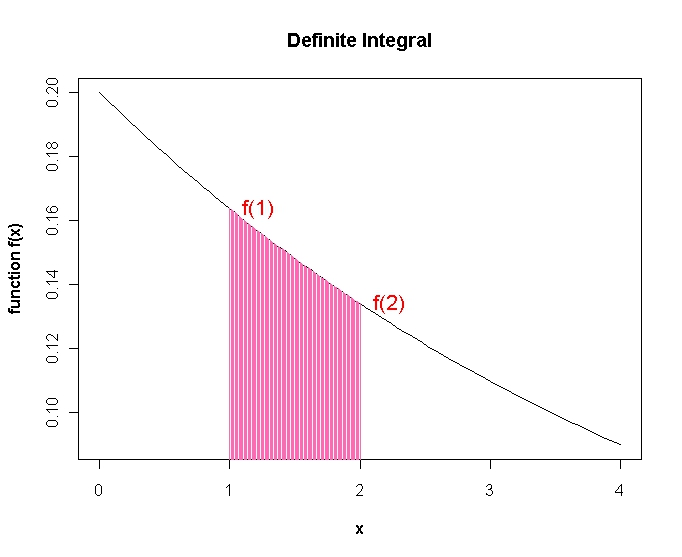
\includegraphics[width=0.5\linewidth]{images/6ADefiniteIntegral}
\caption{Definite integral of function is area under curve between X=1 and X=2.}
\label{fig:6adefiniteintegral}
\end{figure}


%------------------------------------------------------------------------%

\subsection*{Expected Value and Variance}
%---------------------------------------------------------------------%

Here $\lambda > 0$ is the parameter of the distribution, often called the \textbf{rate parameter}. 

The distribution is supported on the interval $[0, \infty)$.The expected value $E(X)$ of an exponentially distributed random variable $X$, specifed with the \textbf{rate parameter} $\lambda$
\[ X \sim \mbox{exp}(\lambda)  \]
is computed using the following formula
\[ E(X) = \frac{1}{\lambda}. \]
The expected value is also known as the exponential mean $\mu$.
\smallskip
\noindent The variance of an exponential random variable $X$ is:
\[\operatorname{Var}(X) = \frac{1}{\lambda^2}\]

\noindent Suppose $\lambda=10$


\[
E(X) = \frac{1}{\lambda} = \frac{1}{1/10} = 10 \]
The variance of an exponential random variable $X$ is:

\[\operatorname{Var}(X) = \frac{1}{\lambda^2} = 100\]





%------------------------------------------------------------------------%


\subsection*{Exponential Distribution: Relationship to Poisson Mean}
\begin{itemize}
\item The Exponential Rate parameter ($\lambda$) is directly related to the Poisson mean (m).
\item If we expect 12 occurrences per hour, then what is the rate of occurrences?
\item We would expected to wait 1/12 of an hour (i.e. 5 minutes) between occurrences.
\item Be mindful to keep your time units consistent, if working with both Poisson and Exponential.
\item If working in minutes, our rate parameter values is $\lambda$ = 0.20 (i.e. 1/5).
%\item (This could be the basis of an exam question).
\end{itemize}




%----------------------------------------------%

% Given that, for an exponential distributed process (where durations are denominated in terms of hours)  the rate parameter is $\lambda$ 




\subsection*{The Memoryless property}
\begin{itemize}
\item The most interesting property of the exponential distribution is the \textbf{\emph{memoryless}} property. 
\item By this , we mean that if  the lifetime of a component is exponentially distributed, then an item which has been in use for some time is a good as a brand new item with regards to the likelihood of failure.
\item 
The exponential distribution is the only distribution that has this property.
\end{itemize}

The exponential distribution is a \textbf{\textit{memoryless distribution}}.

\begin{itemize}
\item Suppose you buy a new mobile phone. What is the probability of a fault within six months?

\item Suppose you have this mobile phone for 12 months. What is the probability of a fault with six months?

\item Under the assumption, the property of being memoryless means that, for both situations, the probability of a fault within six months is the same.

%\item (The assumption of a constant would be unsuitable in many cases)
\end{itemize}



\subsection*{Worked Example}
Suppose that the service time for a customer at a fast-food outlet
has an exponential distribution with mean 3 minutes. What is the probability that a
customer waits more than 4 minutes?

\[ P(X  \leq 4) = 1 -  e^{-4/3} \]

\[ P(X  \geq 4) = e^{-4/3} = 0.2636 \]

%===========================================================================%
\end{document}


%\subsection{The Exponential Distribution}
%A continuous random variable having p.d.f. f(x), where:
%$f(x) = \lambda x e ^{-\lambda x} $
%is said to have an exponential distribution, with parameter $\lambda$. 
%The cumulative distribution is given by:
%$F(x) = 1 – e^{\lambda x}$






% - https://www.soa.org/Files/Edu/edu-exam-p-sample-quest.pdf


%----------------------------------------------%

% Given that, for an exponential distributed process (where durations are denominated in terms of hours)  the rate parameter is $\lambda$ 



% Use the \texttt{R} code on the following slide to help answer these questions.





%
%%------------------------------------------------------------------------%
%
%\noindent \textbf{Exponential Distribution: Example}
%
%As it is CDF values that we are interested in, we use the output from the \texttt{pexp()} commands.
%
%\begin{itemize}
%\item[(a)] $P(X \leq 5)$ = 0.39346934
%\item[(b)] $P(5 \leq X \leq 10)$ \\ = $P( X \leq 10) - P( X \leq 5)$ \\ = 0.63212056- 0.39346934 \\ = 0.2386512 \\= 23.84 $\%$
%\end{itemize}
%
%




\section*{Exponential Probability Distribution}





\subsection{Exponential Distribution Problem}

What is the probability that a customer will spend more than 15 minutes in the bank
\[
P (X > 15) = e ^{-15\lambda}
= e ^{-3 / 2}
= 0.22
\]


What is the probability that a customer will spend more than 15 minutes in the bank given that he is still in the bank after 10 minutes?
\[
P (X > 15|X > 10) = P (X > 5) 
= e ^{-3 / 2}
= 0.604
\]



\section{Important Formulae}

\[
P( X \geq k) =e^{-k}\]
\[
P( X \leq k) = 1 -e^{-k}\]



%% http://www.aiaccess.net/English/Glossaries/GlosMod/e_gm_exponential.htm




%------------------------------------------------------------%




\end{document}
